\documentclass[a4paper,12pt]{article}
\usepackage[utf8]{inputenc}
\usepackage{polski}
\usepackage{graphicx}
\usepackage{amsmath}
\author{}
\title{Efekty termoelektryczne w ciałach stałych}
\begin{document}
\maketitle
\newpage
\section{Wstęp teoretyczny}
Zjawisko termoelektryczne jest to ogól transformacji napięcia elektrycznego i~temperatury. W~zależności od typu zmian, wyróżniamy trzy główne zjawiska:
\begin{description}
\item[zjawisko Seebecka]\hfill \\
	polega na powstawaniu różnicy napięć na stykach dwóch metali, jeżeli dwa styki znajdują się w~różnych temperaturach.
\item[zjawisko Peltiera] \hfill \\
	polega na wydzielaniu się temperatury, bądź jej pochłanianiu na stykach dwóch metali w~wyniku przepływu prądu elektrycznego.
\item[zjawisko Thomsona] \hfill \\
	polega na wydzielaniu się temperatury bądź jej pochłanianiu, w~przewodniku przez który płynie prąd elektryczny, oraz który znajduje się w~różnych temperaturach.
\end{description}

Zjawisko termoelektryczne stosuje się przy generatorach termoelektrycznych.
Generatory takie wykorzystują zjawisko Seebecka.\
Wykonuje się wykorzystując a~pary półprzewodników, z~uwspólnionym potencjałem na jednym biegunie, a~pozostałe bieguny łączone są przez odbiornik energii elektrycznej.
Następnie jeden biegun półprzewodników zostaje podgrzany, a~drugi ochłodzony, aby zmaksymalizować gradient temperatury.
Tak powstałą siłę termoelektryczną możemy odebrać na odbiorniku po zapewnieniu zamkniętego obwodu elektrycznego.

Drugim popularnym urządzeniem wykorzystującym efekty termoelektryczne, jest pompa ciepła.
Wykorzystuje ona zjawisko Peltiera. Układ jest bliźniaczo podobny do generatora termoelektrycznego, jednak zamiast odbiornika energii, mamy źródło napięciowe.
Po wymuszeniu różnicy napięć, a~co za tym idzie, przepływu prądu elektrycznego, na łączeniach półprzewodników następuje chłodzenie oraz grzanie.
W~zależności od potrzeb, wykorzystujemy biegun pochłaniający ciepło w~celu chłodzenia, bądź biegun oddający ciepło w~celu grzania.

Siła termoelektryczna jest wielkością obrazującą wielkość napięcia powstającego pod wpływem gradientu temperatury.
Wielkość siły termoelektrycznej jest zależna typu materiału.\\
Ogólny wzór na siłę termoelektryczną przyjmuje postać:
$$\alpha=\dfrac{k_B}{e}\int\left(\dfrac{E-E_F}{k_BT}\right)\dfrac{\sigma(E)}{\sigma}dE$$
Opracowane wzory skrócone, ze względu na typ przewodnika, i~przyjmują one następujące postaci:
\begin{description}
\item[metale i~półprzewodniki zdegenerowane]\hfill \\
	$\alpha=\dfrac{\pi^2k_BT}{3eE_F}$
\item[półprzewodniki samoistne]\hfill \\
$\alpha=\dfrac{k_B}{e}\dfrac{\mu_n-\mu_p}{\mu_n+\mu_p}\left(2+\dfrac{E_g}{2k_BT}\right)$
\item[półprzewodniki domieszkowe]\hfill \\
$\alpha=\dfrac{k_B}{e}\left(-\dfrac{E_F}{k_BT}+r+\dfrac{5}{2}\right)$
\end{description}
\section{Opracowanie wyników}
\subsection{Temp: 350$^\circ$C}
\begin{tabular}{|c|c|c|c|c|c|c|c|}
\hline
L.p&$T_1$mV&$T_2$mV&$T_1^\circ$C&$T_2^\circ$C&$\Delta T^\circ$C&V mV&$\Delta V$ mV\\
\hline
1&3.671&3.671&442.7&442.7&0.0&0.708&0\\
2&3.688&3.670&444.5&442.6&1.9&1.152&0.444\\
3&3.701&3.670&445.9&442.6&3.3&1.483&0.775\\
4&3.711&3.670&446.8&442.6&4.2&1.169&0.461\\
5&3.719&3.671&447.5&442.7&4.8&1.185&0.477\\
6&3.726&3.671&448.3&442.7&5.6&2.010&1.302\\
7&3.731&3.671&449.0&442.7&6.3&2.400&1.692\\
8&3.735&3.672&449.3&442.9&6.4&2.220&1.512\\
9&3.739&3.383&449.7&443.0&6.7&2.310&1.602\\
10&3.743&3.673&450.0&443.0&7.0&2.369&1.661\\
\hline
\end{tabular}\\
\begin{center}
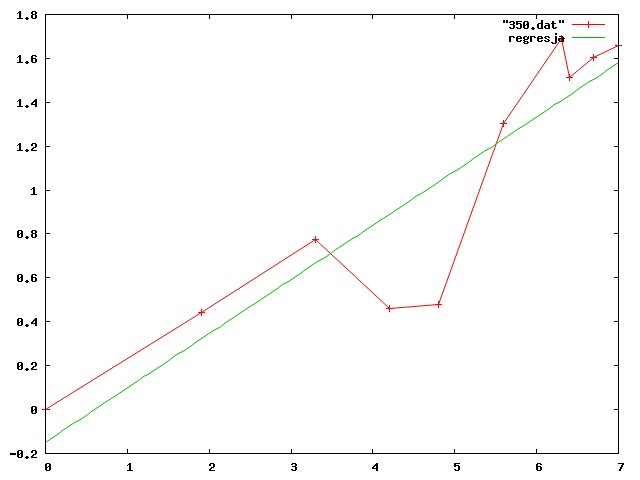
\includegraphics[width=400px]{350}
\end{center}

Wartość siły termoelektrycznej: 0.246
\subsection{Temp: 370$^\circ$C}
\begin{tabular}{|c|c|c|c|c|c|c|c|}
\hline
L.p&$T_1$mV&$T_2$mV&$T_1^\circ$C&$T_2^\circ$C&$\Delta T^\circ$C&V mV&$\Delta V$ mV\\
\hline
1&3.760&3.752&451.8&451.0&0.8&0.879&0.000\\
2&3.775&3.752&453.4&451.0&2.4&1.119&0.240\\
3&3.785&3.753&454.5&451.0&3.5&1.417&0.538\\
4&3.797&3.754&455.7&451.2&4.5&1.638&0.759\\
5&3.805&3.755&456.5&451.4&4.9&1.814&0.935\\
6&3.811&3.756&457.0&451.4&5.6&1.943&1.064\\
7&3.817&3.757&457.7&451.5&6.2&2.043&1.164\\
8&3.822&3.758&458.1&451.6&6.5&2.119&1.240\\
9&3.826&3.759&458.5&451.7&6.8&2.193&1.314\\
10&3.830&3.760&459.0&451.8&7.2&2.247&1.368\\
\hline
\end{tabular}\\
\begin{center}
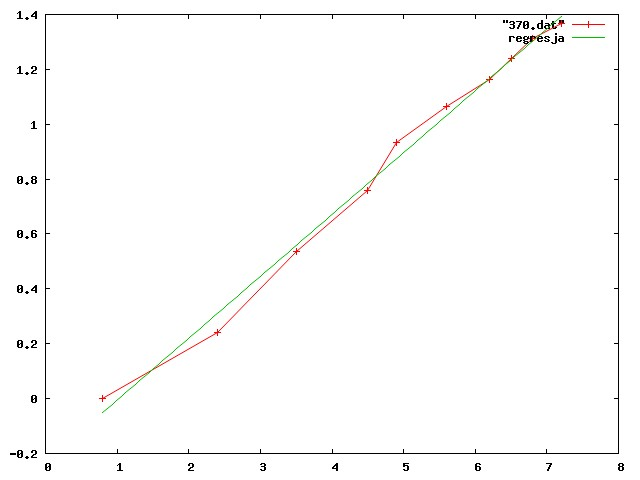
\includegraphics[width=400px]{370}
\end{center}

Wartość siły termoelektrycznej: 0.225
\subsection{Temp: 390$^\circ$C}
\begin{tabular}{|c|c|c|c|c|c|c|c|}
\hline
L.p&$T_1$mV&$T_2$mV&$T_1^\circ$C&$T_2^\circ$C&$\Delta T^\circ$C&V mV&$\Delta V$ mV\\
\hline
1&3.903&3.904&466.5&466.5&0.0&0.524&0.000\\
2&3.920&3.904&468.1&466.5&1.6&0.930&0.406\\
3&3.931&3.905&469.4&466.6&2.8&1.196&0.672\\
4&3.942&3.905&470.5&466.6&3.9&1.376&0.852\\
5&3.950&3.906&471.4&466.8&4.6&1.527&1.003\\
6&3.956&3.907&472.0&466.9&5.1&1.643&1.119\\
7&3.962&3.908&472.5&467.0&5.5&1.742&1.218\\
8&3.967&3.909&473.0&467.1&5.9&1.834&1.310\\
9&3.972&3.910&473.5&467.2&6.3&1.897&1.373\\\
10&3.972&3.912&473.5&467.4&6.1&1.967&1.443\\
\hline
\end{tabular}\\
\begin{center}
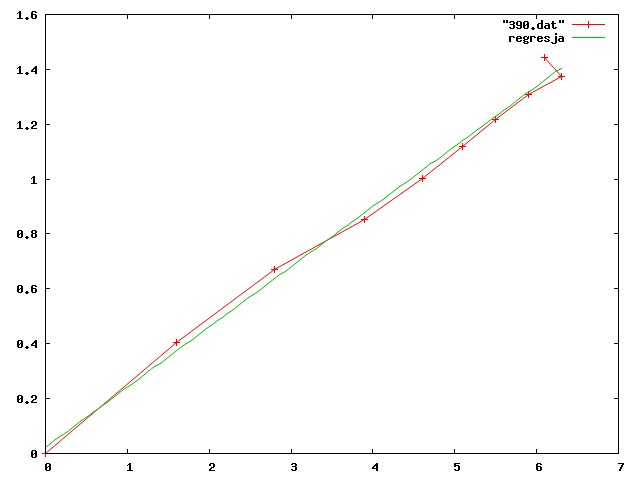
\includegraphics[width=400px]{390}
\end{center}

Wartość siły termoelektrycznej: 0.219
\subsection{Temp: 410$^\circ$C}
\begin{tabular}{|c|c|c|c|c|c|c|c|}
\hline
L.p&$T_1$mV&$T_2$mV&$T_1^\circ$C&$T_2^\circ$C&$\Delta T^\circ$C&V mV&$\Delta V$ mV\\
\hline
1&4.099&4.113&486.3&487.8&-1.5&-0.124&0.000\\
2&4.103&4.112&486.8&487.7&-0.9&-0.293&0.169\\
3&4.110&4.111&487.6&487.6& 0.0& 0.527&0.651\\
4&4.121&4.110&488.7&487.5& 1.2& 1.702&1.826\\
5&4.130&4.110&489.6&487.5& 2.1& 1.912&2.036\\
6&4.140&4.110&490.5&487.5& 3.0& 2.099&2.223\\
7&4.148&4.110&491.4&487.5& 3.9& 2.264&2.388\\
8&4.156&4.110&492.4&487.5& 4.9& 2.398&2.522\\
9&4.161&4.110&492.7&487.5& 5.2& 2.494&2.618\\
10&4.166&4.110&493.3&487.5&5.8& 2.591&2.715\\
\hline
\end{tabular}\\
\begin{center}
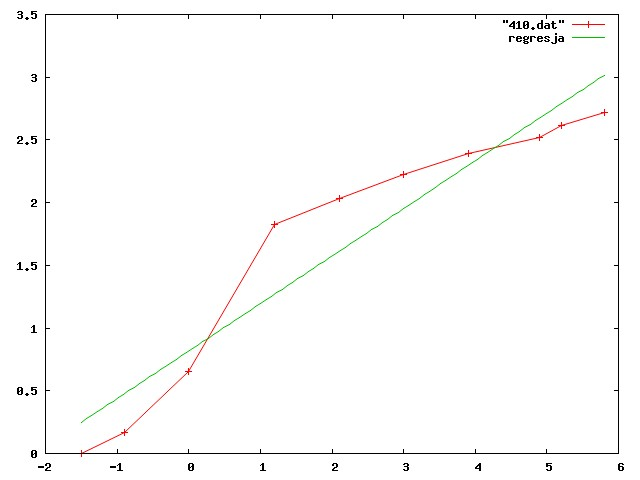
\includegraphics[width=400px]{410}
\end{center}

Wartość siły termoelektrycznej: 0.379

\subsection{Siła termoelektryczna}
\begin{center}
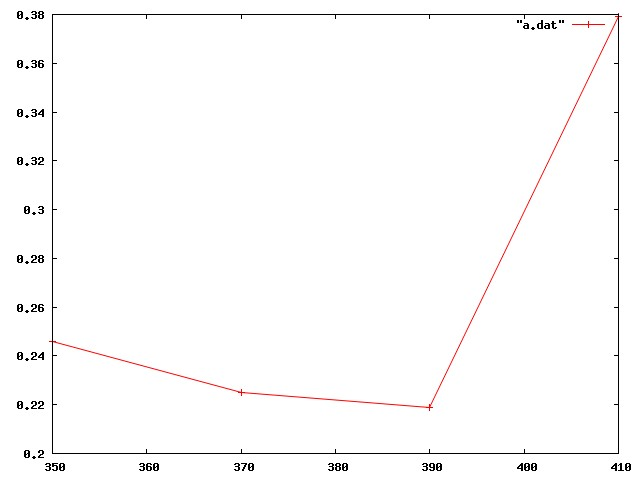
\includegraphics[width=400px]{a}
\end{center}
\subsection{Ułamkowa zależność obsadzenia dostępnych położeń}
$\alpha=\dfrac{k_B}{e}\ln\dfrac{c_0-c}{c}$\\
$\dfrac{\alpha* e}{k_B}=\ln\dfrac{c_0-c}{c}$\\
$\dfrac{c_0-c}{c}=e^{\dfrac{\alpha * e}{k_B}}$\\
$\dfrac{c_0}{c}=1+e^{\dfrac{\alpha * e}{k_B}}$\\
\begin{description}
\item[350]\hfill \\
$alpha=0.246$\\
$\dfrac{c}{c_0}=0.0544$
\item[370]\hfill \\
$alpha=0.225$\\
$\dfrac{c}{c_0}=0.0684$
\item[390]\hfill \\
$alpha=0.219$\\
$\dfrac{c}{c_0}=0.0730$
\item[410]\hfill \\
$alpha=0.379$\\
$\dfrac{c}{c_0}=0.0121$
\end{description}
\begin{center}
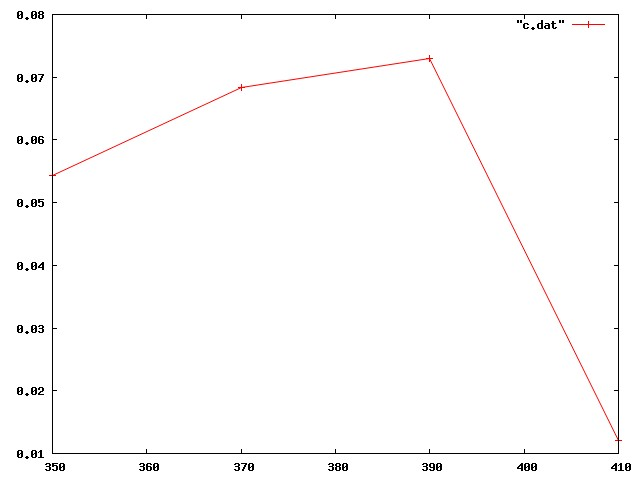
\includegraphics[width=400px]{c}
\end{center}

\end{document}
